\section{Performance}

As mentioned previously, the user must specify the requested cluster count \textit{k}. To to find a suitable value for \textit{k}, the user will need to trial a number of values. To minimize any negative effect on user-experience it is important, therefore, that the clustering performs in near real-time, irrespective of terrain size and cluster count.\\

The performance of the CPU and GPU clustering implementations are analysed below along with an evaluation of the GPU speed-up. In order to evaluate the performance of the different implementations, the clustering time is analysed in relation to terrain size and cluster count. In order to accurately compare their performance, the same terrains are used with identical resources specified. In these tests, the maximum value of \textit{K} is set to ten. Although the system permits users to generate up to fifty clusters, ten is deemed sufficient for most use cases. All tests were performed on a machine with specifications outlined in appendix \ref{AppendixD}.

\begin{figure}
\center
	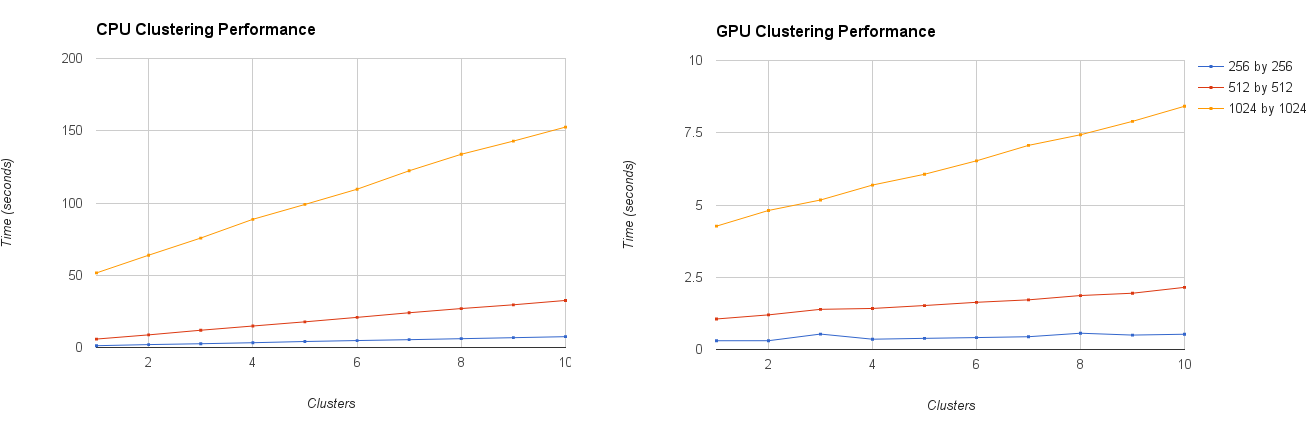
\includegraphics[width=\textwidth]{clustering_performance_aggregate.png}
	\caption{ Time it takes for the clustering process to complete on the CPU (left) and GPU (right) in relation to the number of clusters. The analysis was performed for terrains of size: 256 by 256 (blue), 512 by 512 (red) and 1024 by 1024 (orange).}	
	\label{fig:aggregate_clustering_performance}
\end{figure}

\subsection{CPU Performance}

Figure \ref{fig:aggregate_clustering_performance} shows the clustering time achieved on the CPU for different terrain sizes and number of clusters. From this data, it is possible to conclude that the clustering time increases linearly with the number of clusters and the clustering time is proportional to terrain area.

Although the clustering time is reasonable for smaller terrains, this processing time increases sharply with terrain size. This is especially true when combined with an increase in the number of clusters to generate. Generating ten clusters on a large terrain (1024 by 1024) takes just over 2.5 minutes.

\subsection{GPU Performance}

Figure \ref{fig:aggregate_clustering_performance} illustrates the performance of the same tests run on the GPU. From this data, it is possible to conclude that the processing time increases linearly with cluster count but at a significantly slower rate than on the CPU. This is because individual clusters are managed in parallel on the GPU. Also, similarly to the CPU implementation, the processing time increases linearly with terrain area. Unlike the cluster count, however, the rate of increase is comparable to that of the CPU implementation. The reason for this is because, although individual terrain vertices are managed in parallel on the GPU implementation, the number of vertices far outweighs the number of GPU cores. 

\subsection{GPU Speed-up}

Figure \ref{fig:clustering_cpu_v_gpu_speedup} shows the GPU clustering speed-up over CPU for square terrains of size 256, 512 and 1024, respectively. These graphs show that the GPU significantly outperforms the CPU, irrespective of terrain size and cluster count. \\
Also visible is the increased sensitivity to cluster count of the CPU implementation over the GPU (speed-up increases with respect to cluster count). \\
This graph also shows that the GPU speed-up increases with terrain size. Because each terrain vertex is processed by a separate thread in the GPU clustering algorithm, increasing the number of vertices will accentuate the GPU acceleration. \\

\begin{figure}
\center
	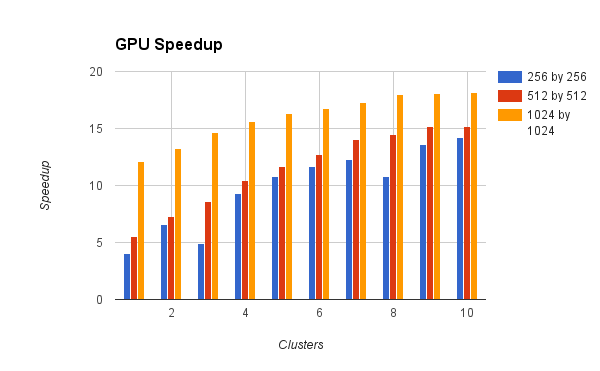
\includegraphics[width=\textwidth]{clustering_cpu_v_gpu_speedup.png}
	\caption{ Calculated clustering speed-up of the GPU over CPU implementation for square terrains of size 256 by 256 (blue), 512 by 512 (red) and 1024 by 1024(yellow).}	
	\label{fig:clustering_cpu_v_gpu_speedup}
\end{figure}